\documentclass[border=6pt]{standalone}
\usepackage{fontspec,xeCJK,amsmath,amssymb,tikz,graphicx}
\usetikzlibrary{arrows.meta}
\setmainfont{Arial}\setCJKmainfont{PingFang SC}
\definecolor{ink}{HTML}{203340}\definecolor{blue}{HTML}{147E91}\definecolor{pale}{HTML}{EFF6F5}\definecolor{line}{HTML}{D3E0DF}\definecolor{warm}{HTML}{BA652C}
\begin{document}\begin{tikzpicture}[x=1cm,y=1cm,every node/.style={text=ink,font=\fontsize{10}{13}\selectfont},flow/.style={-{Stealth[length=5pt]},draw=blue,line width=1pt}]
\path[use as bounding box](0,0)rectangle(11,29.2);\fill[pale](0,0)rectangle(11,29.2);
\node[font=\fontsize{19}{23}\selectfont\bfseries]at(5.5,28.4){SAM：提示怎样变成像素区域};
\node[text=blue]at(5.5,27.7){图像缓存复用；提示与图像双向交互};
\draw[rounded corners=6pt,draw=line,fill=white](.35,22.2)rectangle(10.65,27.0);
\node[anchor=west,font=\fontsize{13}{16}\selectfont\bfseries]at(.65,26.45){A　图像缓存};
\node at(2.15,24.3){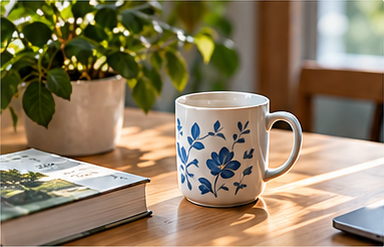
\includegraphics[width=2.8cm,height=2.7cm,keepaspectratio]{visual-1.png}};
\node[anchor=west]at(3.8,25.5){输入：1024$\times$1024 图像};
\node[anchor=west]at(3.8,24.78){ViT-H/16 $\to$ 卷积调整通道};
\node[anchor=west]at(3.8,24.06){缓存 $E:64\times64\times256$};
\node[anchor=west]at(3.8,23.34){新点击复用缓存；对应正文 §3.1};
\draw[flow,dotted](5.5,22.2)--(5.5,21.8);
\draw[rounded corners=6pt,draw=line,fill=white](.35,17.0)rectangle(10.65,21.8);
\node[anchor=west,font=\fontsize{13}{16}\selectfont\bfseries]at(.65,21.25){B　提示编码};
\node at(2.15,19.1){
\includegraphics[width=2.8cm,height=2.7cm,keepaspectratio]{visual-2.png}};
\node[anchor=west]at(3.8,20.3){点/框：位置 + 类型 $\to$ 256维 token};
\node[anchor=west]at(3.8,19.580000000000002){粗掩码：256$^2\to64^2\times256$};
\node[anchor=west]at(3.8,18.86){密集特征加到 E；稀疏 token 进 C};
\node[anchor=west]at(3.8,18.14){对应正文 §2、§3.2};
\draw[flow,dotted](5.5,17.0)--(5.5,16.6);
\draw[rounded corners=6pt,draw=line,fill=white](.35,11.8)rectangle(10.65,16.6);
\node[anchor=west,font=\fontsize{13}{16}\selectfont\bfseries]at(.65,16.05){C　双向解码};
\node at(2.15,13.900000000000002){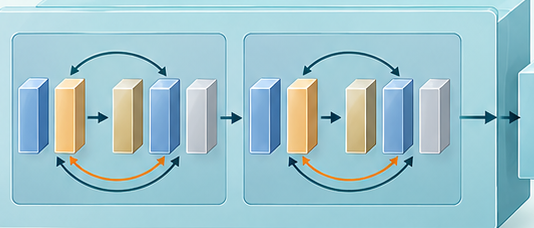
\includegraphics[width=2.8cm,height=2.7cm,keepaspectratio]{visual-3.png}};
\node[anchor=west]at(3.8,15.100000000000001){token 自注意力 $\to$ token读图像};
\node[anchor=west]at(3.8,14.38){前馈变换 $\to$ 图像读token；重复2层};
\node[anchor=west]at(3.8,13.660000000000002){上采样 $U:256\times256\times32$};
\node[anchor=west]at(3.8,12.940000000000001){mask token $\to w_k\in\mathbb R^{32}$；$M_k=U w_k$};
\draw[flow,dotted](5.5,11.8)--(5.5,11.4);
\draw[rounded corners=6pt,draw=line,fill=white](.35,6.599999999999999)rectangle(10.65,11.399999999999999);
\node[anchor=west,font=\fontsize{13}{16}\selectfont\bfseries]at(.65,10.849999999999998){D　训练与纠错};
\node at(2.15,8.7){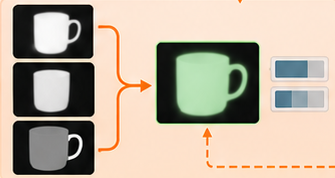
\includegraphics[width=2.8cm,height=2.7cm,keepaspectratio]{visual-4.png}};
\node[anchor=west]at(3.8,9.899999999999999){三个候选；最低 mask loss 反传};
\node[anchor=west]at(3.8,9.179999999999998){预测 IoU 辅助选择；模拟11轮交互};
\node[anchor=west]at(3.8,8.459999999999999){GT比较 $\to$ 梯度更新 A/B/C};
\node[anchor=west]at(3.8,7.739999999999998){对应正文 §3.4；推理时参数固定};
\draw[flow,dotted](5.5,6.599999999999999)--(5.5,6.199999999999998);
\draw[rounded corners=6pt,draw=line,fill=white](.35,1.3999999999999995)rectangle(10.65,6.199999999999999);
\node[anchor=west,font=\fontsize{13}{16}\selectfont\bfseries]at(.65,5.6499999999999995){E　数据引擎};
\node at(2.15,3.499999999999999){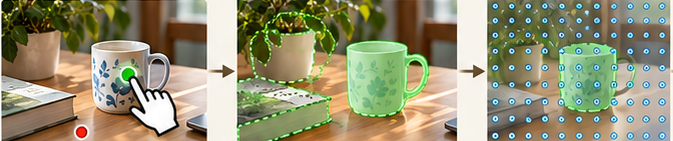
\includegraphics[width=2.8cm,height=2.7cm,keepaspectratio]{visual-5.png}};
\node[anchor=west]at(3.8,4.699999999999999){人工辅助 $\to$ 半自动补漏 $\to$ 自动};
\node[anchor=west]at(3.8,3.9799999999999995){网格点生成；质量/稳定性筛选；去重};
\node[anchor=west]at(3.8,3.2599999999999993){数据回到 D 训练，模型再帮标注};
\node[anchor=west]at(3.8,2.539999999999999){§4--5讲数据；§6检验 A/B/C 的效果};
\end{tikzpicture}\end{document}